\chapter{Evaluation \& Results}

\section{Carpark Tests}




%%%%%%%%%%%%%%%%%%%%%%%%%%%%%%%%%%%%%%%%
\begin{figure}[h]
      \centering
      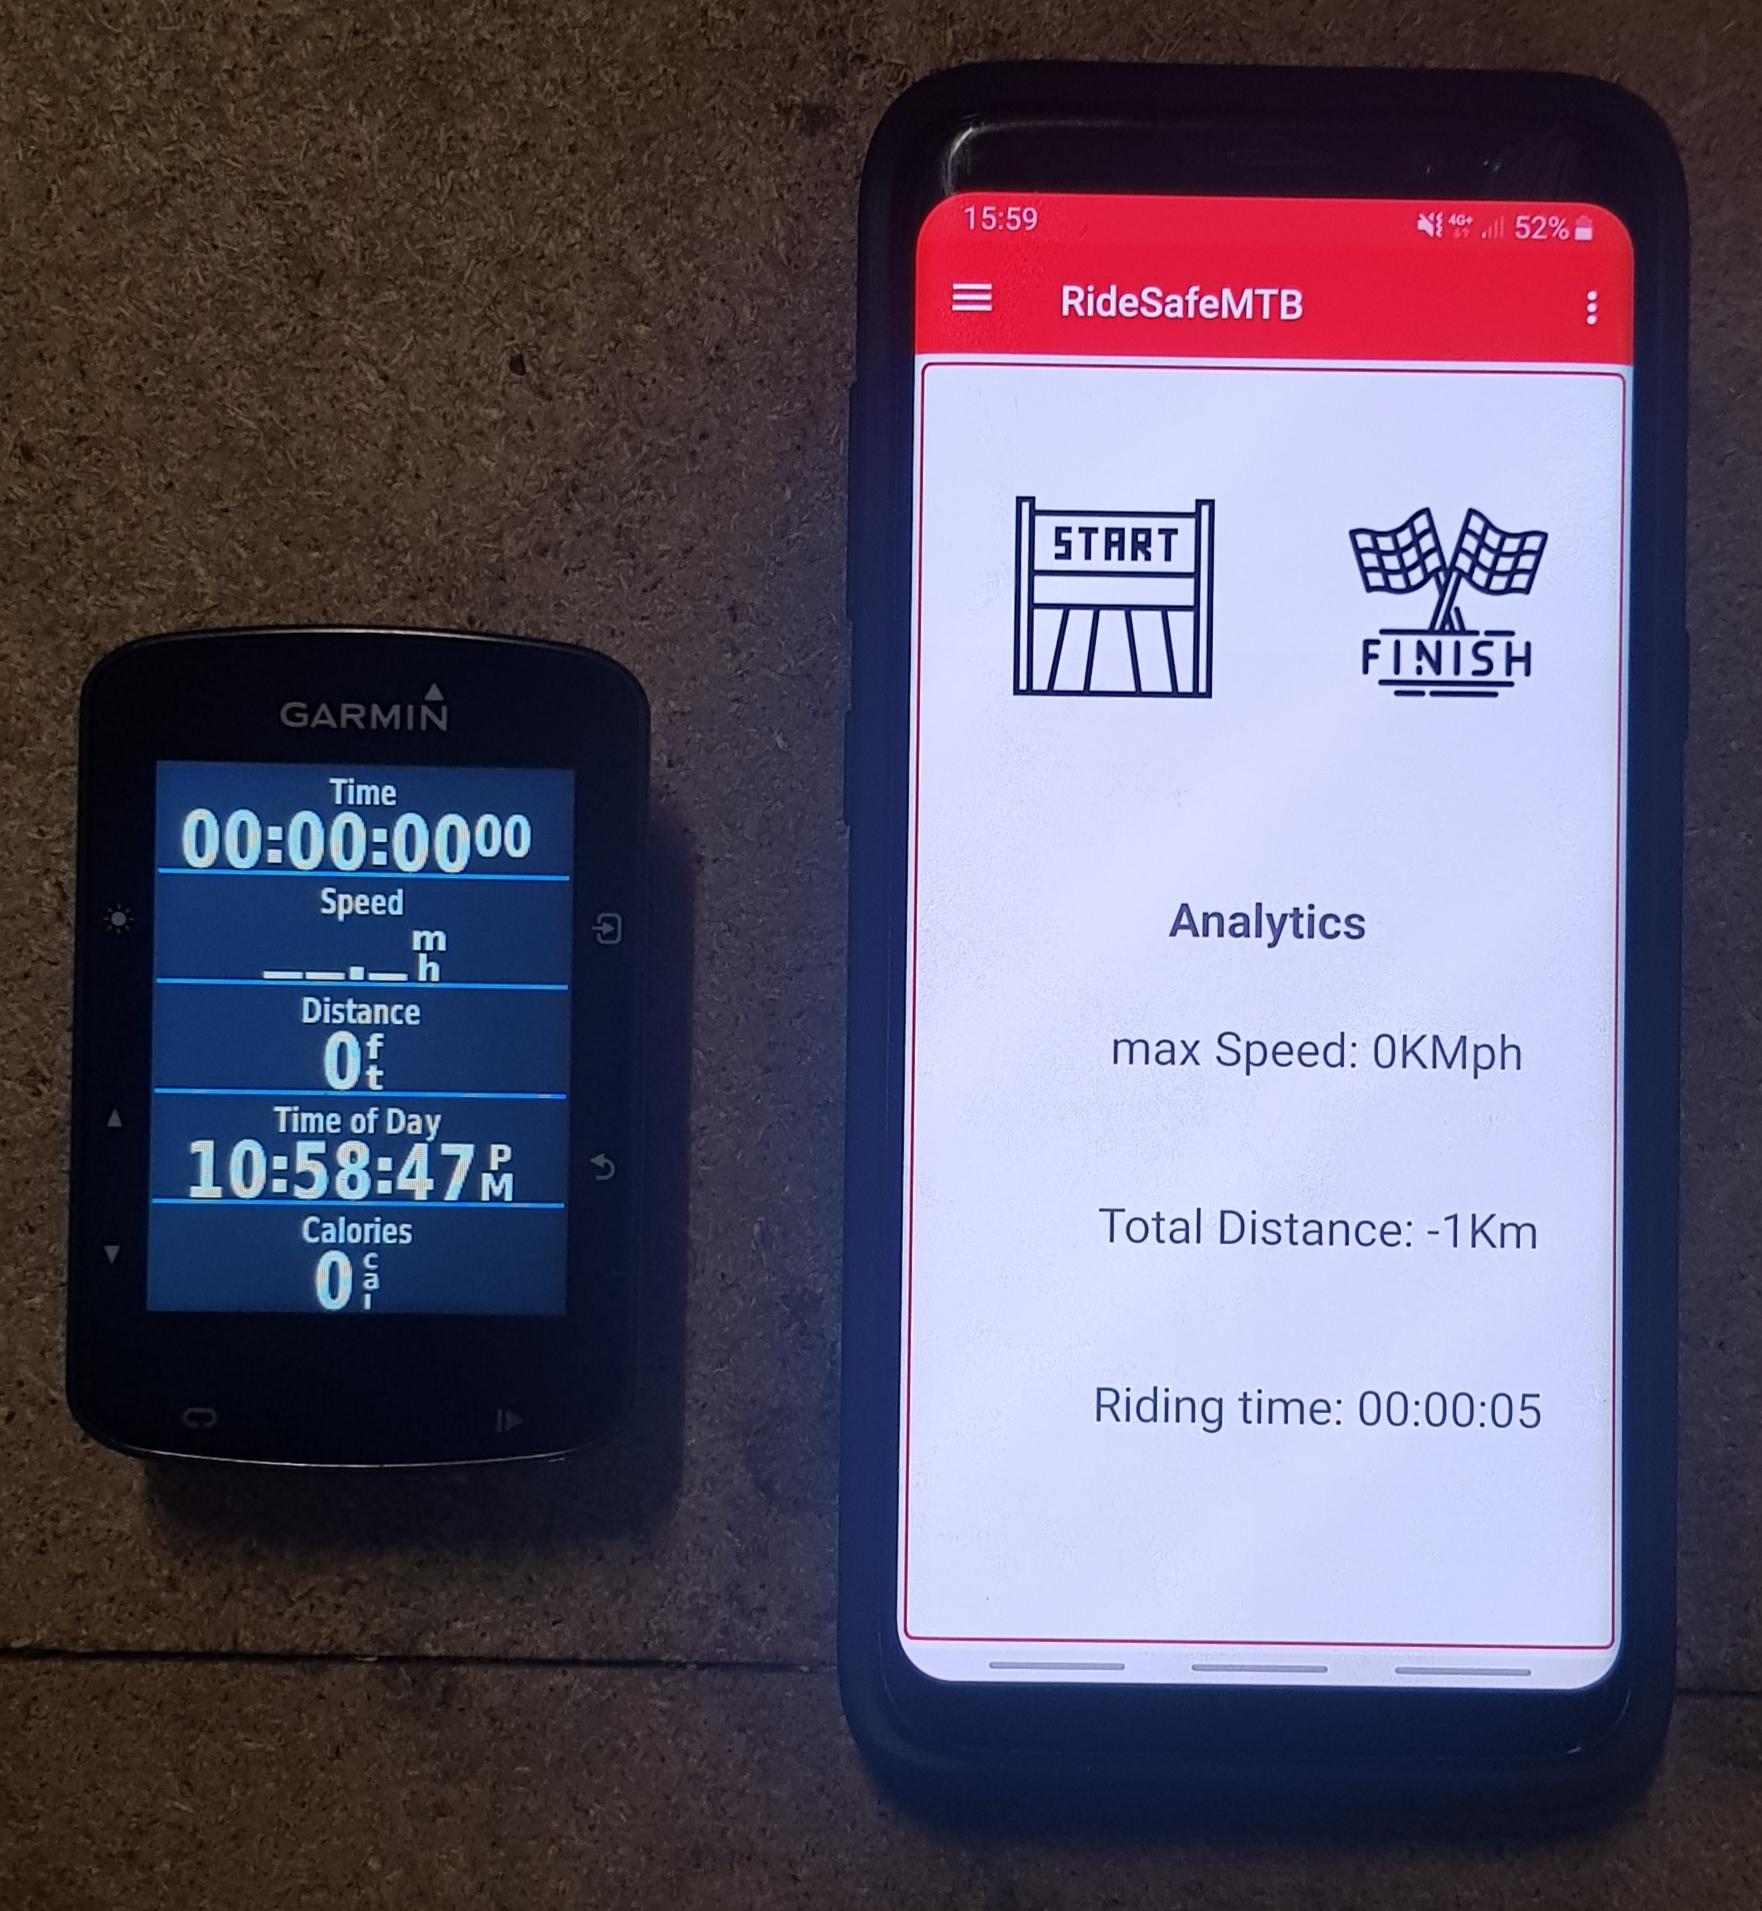
\includegraphics[scale = .1]{evaluation/gvr.jpg}
      \caption{Garmin Edge 520 Vs RideSafe (Samsung Galaxy s8)}
      \label{trail}
\end{figure}
%%%%%%%%%%%%%%%%%%%%%%%%%%%%%%%%%%%%%%%%


From analyzing user reports of existing solutions three common issues arose, issues impacting the user experience enough for users to abandon using the systems altogether. 
RideSafe installed on a Samsung Galaxy s8 was tested side by side with Garmin Edge 520.
Each test was carried out 10 times.

\begin{itemize}
\item Drop Test
\end {itemize}

The drop test consisted of dropping both devices side by side from hip height, onto a wooden floor.


\begin{itemize}
\item Hard Braking
\end {itemize}

The hard braking test was performed with each device in a trouser pocket, pedaling up to an average speed of 25km/h and coming to a complete stop as quickly as possible.



\begin{itemize}
\item Shake Test
\end {itemize}

The shake test was conducted by putting both devices in hand and shaking vigorously for a random amount of time each run.




The results of these “carpark Tests” are shown in table \ref{cpt} . The number present in each cell is the number of times the system failed and detected a crash.


\begin{table}
\caption{Carpark Tests}
\label{cpt}
\begin{center}
 \begin{tabular}{||c | c |c||} 
 \hline
 Test Type & RideSafe & Garmin Edge 520 \\ [0.5ex] 
 \hline\hline
 Drop Test & 0 & 6 \\ 
 \hline
 Hard Braking & 1 & 4\\
 \hline
 Shake Test  & 0 & 10 \\ [1ex] 
 \hline
\end{tabular}
\end{center}
\end{table}




\section{Real World Testing}


The main real world tests of the system were conducted on two seperate days,in two seperate locations. Ridesafe was evaluated by recording the number of accidents reported by the application vs the true number of accidents which may have occurred. Participants with a personal relationship to the author may also be included as participants. The procedure for the testing was as follows:

\begin{itemize}


\item 1 Install the application.
\item 2 Before commencing a run start the background service by pressing “start” on the home screen.
\item 3 upon completion of the cycle the service was stopped.
\item 4 The number of detected crashes displayed on the settings screen was noted.
\item 5 The true number of crashes detected was recorded.
\end {itemize}

\subsection*{Testing Day one}

The First test of RideSafe were conducted by 4 participants of varying skill including the author. Testing was conducted on “Red” “Black” and uncategorized trails located on Ticknock mountain Co. Dublin. Testing took place over a 2 hour period consisting of on average 6 runs per rider. The test results from day one are shown in Table \ref{day1}.

\vspace{1cm}
\begin{table}
\caption{Testing Day 1: Results}
\label{day1}
\begin{center}
 \begin{tabular}{||c |c |c ||} 
 \hline
 Rider \# & No of Actual Crashes & Number of Detected Crashes \\ [0.5ex] 
 \hline\hline
 1& 0 & 0 \\ 
 \hline
 2& 1 & 0 \\ 
 \hline
 3 & 0 & 0\\
 \hline
4 & 0 & 0 \\ [1ex] 
 \hline
\end{tabular}
\end{center}
\end{table}

\vspace{1cm}
Findings from testing day one provided interesting insights to the operation of the performance of RideSafe, Rider \#2 briefly lost control and veered off the trail for a couple of moments, without actually falling of the bicycle. As the rider considered this a crash (albeit very minor) the result was recorded. As RideSafe is trained to detect more severe crashes where there is a potential for injury I can conclude RideSafe correctly did not flag this as a crash. No false positives were detected in day one of testing.


\subsection*{Testing Day Two}

For testing day two more participants were required to accurately evaluate the system.
With permission to recruit participants having being granted by the owners, Testing Day 2 took place at Glencullen Adventure Park. Glencullen Adventure Park offers a more diverse selection of trails, more indicative to what is commonly ridden around ireland ranging from smooth flowy trails (left) to intense rough technical trails(Right) as shown in figure \ref{trail}.


%%%%%%%%%%%%%%%%%%%%%%%%%%%%%%%%%%%%%%%%
\begin{figure}[h]
      \centering
      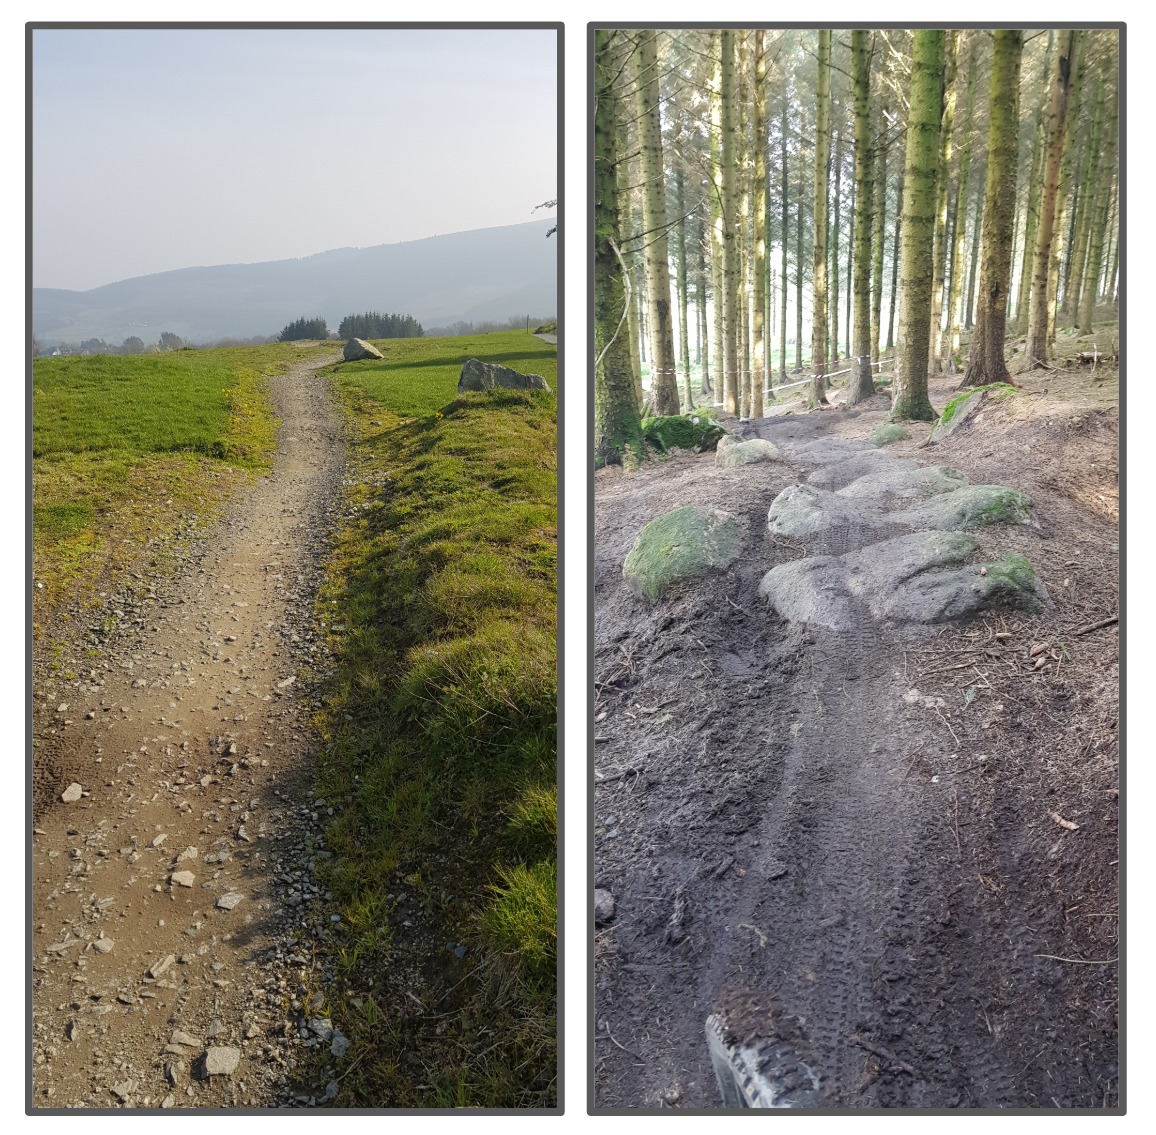
\includegraphics[scale = .5]{evaluation/trails.png}
      \caption{A Smooth trail (left) vs A steep technical trail (Right)}
      \label{trail}
\end{figure}
%%%%%%%%%%%%%%%%%%%%%%%%%%%%%%%%%%%%%%%%


Being restricted to recruit participants over the age of 18, who have a compatible android phone and cycle with their phone on their person the author managed to recruit 12 willing participants in total. Participants recruited were of all skill levels and ages. The author while personally participating exported RideSafes database upon completing a full run while top to bottom, the total count of exported databases was used to calculate the average number of runs completed per rider. Results have been calculated on both a per rider basis as well as per total estimated run count.  Results are listed separately and clearly labeled. 
  



\begin{table}
\caption{Testing Day 2: Per Rider Results}
\label{day2}
\begin{center}

 \begin{tabular}{||c| c| c| c| c||} 

 \hline
 Rider \# & No of Actual Crashes & Number of Detected Crashes & False Positives  & Missed Detections\\ [0.5ex] 
 \hline\hline
 1 & 0 & 0 & 0 & 0 \\ 
 \hline
2 & 0 & 0 & 0 & 0\\ 
 \hline
3 & 0 & 0 & 0 & 0\\ 
 \hline
4 & 0 & 0 & 0 & 0\\ 
 \hline
5 & 3 & 2 & 0 & 1\\ 
 \hline
6 & 0 & 0 & 0 & 0\\ 
 \hline
7 & 0 & 0 & 0 & 0\\ 
 \hline
8 & 1 & 1 & 0 & 0\\ 
 \hline
9 & 0 & 0 & 0 & 0\\ 
 \hline
10 & 0 & 2 & 2 & 0\\ 
 \hline
11 & 1 & 1 & 0 & 0\\ 
 \hline
12 & na & na & na & na\\ [1ex] 
 \hline
\end{tabular}
\end{center}
\end{table}
\vspace{1cm}


Out of 12 willing participants one participant left without debriefing so as a result their results are not available(Rider \#12). 

\begin{itemize}
\item Out of 5 reported crashes occurring RideSafe correctly identified 80\% of them ( True Detections).
\end {itemize}

Rider \#5 reported 3 accidents occurring while using the application, 2 of which were detected.
Rider \#8 reported 1 accident occurring which was correctly identified.
Rider \#11 reported 1 accident occurring which was correctly identified.

\begin{itemize}
\item Rider \#10 reported no accidents had occurred while using RideSafe however two incorrect  
detections were made resulting in two False Positives.
\end{itemize}

\vspace{2cm}

\begin{table}
\caption{Per Rider System Results}
\label{sr}
\begin{center}
 \begin{tabular}{||c| c|  c||} 
 \hline
 True Detection Accuracy & False Positive Percentage & Missed Detection \\ [0.5ex] 
 \hline\hline
  80\% & 18.1\% & 9\% \\ [1ex] 
 \hline
\end{tabular}
\end{center}
\end{table}




The total number of recorded runs as completed by the author were 9 compete runs.
Using this number \[ 9 \pm 1 \] the total number of runs was estimated as : 


\[ \frac{((11\cdot8) + (11\cdot9) + (11\cdot10))}{3} = 99 \]

With one rider experiencing two false positives the percentage can be calculated as \[ \frac{2}{99} \cdot \frac{100}{1} = 2.02\% \] 









Concerning the crashes reported vs detected crashes ,the author is led to believe the  test methodology is partly to blame, What is the definition of a crash? Is an injury required to constitute a crash?  Leaving these questions unanswered led to participants having their own definition of what exactly is considered a crash, this is the number which was reported to the author. RideSafe being trained on more serious crashes which would cause an injury by design, should not detect very minor incidents leading the author to believe the missed detections are from very minor incidents.

In relation to the false positives detected while Rider \# 10 was testing, the author believes they were caused by one of two reasons:

\subsection *{Unsatisfactory hardware / Gps connectivity}

As RideSafe rule based system is heavily influenced by the requirement of the riders current speed, in the case of both no GPS reception and bad network signal speed will not be possible to compute. The combination of an impact paired with the loss of being able to calculate speed could trigger the crash detection algorithm.


\subsection*{Unsuitable Training Data}
As the system was mainly trained solely by the author, it is probable the model is unsuitable for every type of rider, the model will evolve over time as crashes are recorded by individuals but all the testing was conducted using the same model. Riders riding bikes without adequate suspension dampening would also experience more forces than riders with adequate suspension.




\newpage



\section{Application Performance}




The performance of RideSafe is of utmost importance. For the target audience the issue of battery life can result in the difference between life and death. With ones mobile phone being rendered utterly useless with a dead battery, the efficiency of ridesafe has been thoroughly tested.RideSafe’s performance in terms of power consumption was evaluated using Android studio's built in profiling tool. Figure \ref{load} highlights the performance of RideSafe during the training phase and when idle. Spikes of medium power consumption can be observed in the “splash Screen” where in this case firstly the training data is being read from a file and stored in a database, followed by the training of the logistic regression model. As this process is rarely called the impact on battery life is not concerning. As the application is left idle it uses negligible amounts of system resources ( >2\% CPU usage \& circa 200MB of RAM).

%%%%%%%%%%%%%%%%%%%%%%%%%%%%%%%%%%%%%%%%
\begin{figure}[h]
      \centering
      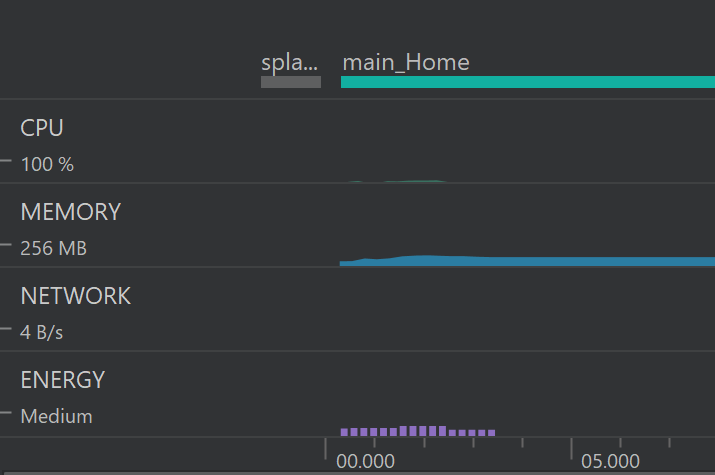
\includegraphics[scale = 1]{evaluation/load.png}
      \caption{Resource utilization during Training / idle}
      \label{load}
\end{figure}
%%%%%%%%%%%%%%%%%%%%%%%%%%%%%%%%%%%%%%%%




Figure \ref{service} shows the performance of RideSafe when the background service is running. CPU and Memory usage remain consistently low while the service is running. Optimisations such as keeping the contents of the service to only what is absolutely necessary for the functional requirements to be implemented. The use of a background activity itself with no visualizations on screen has been shown to conserve power itself as on of the biggest battery drains on an android device is the screen itself \cite{power}.   Spikes of energy can be observed over time as the service runs due to the calculation of speed via GPS. The calculations required for GPS are unfortunately expensive in terms of battery consumption. As speed is crucial to the operation of RideSafe, its removal is currently not possible, but as will be discussed in the following chapter a possible solution does exist. Overall the power consumption of ridesafe is considered to be classified as Low-Medium.

%%%%%%%%%%%%%%%%%%%%%%%%%%%%%%%%%%%%%%%%
\begin{figure}[h]
      \centering
      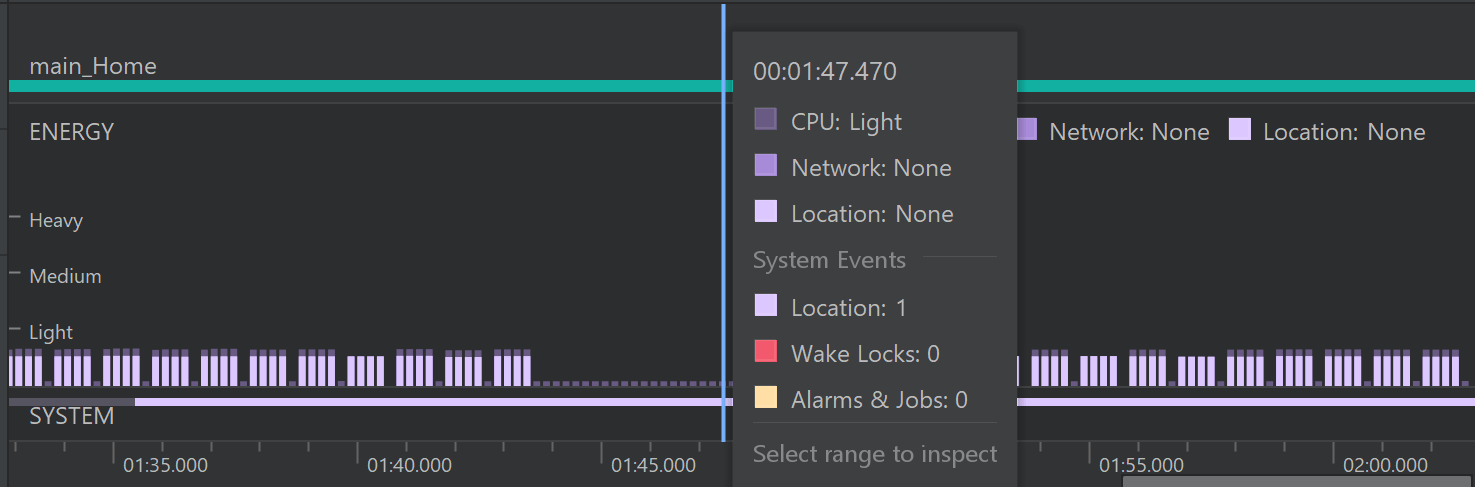
\includegraphics[scale = .8]{evaluation/service.png}
      \caption{Background Service Performance}
      \label{service}
\end{figure}
%%%%%%%%%%%%%%%%%%%%%%%%%%%%%%%%%%%%%%%%
